\documentclass[11pt]{article}
\usepackage{hyperref}
\usepackage{natbib}
\usepackage{amsmath}
\usepackage{nicefrac}
\usepackage[usenames,dvipsnames]{xcolor}
\usepackage{graphicx}
\usepackage{footnote}
\usepackage{rotating}
\usepackage{slashbox}
\usepackage{afterpage}
\usepackage{float}
\citestyle{apj}
%%%%%%%%%%%%%%%%%%%%%%%%%%%%%%%%%%%%%%%%%%%%%%%%%%%%%%%%%%%%%%%%%%%%%%%%%%%%
%force setting figures at the top of the page:
    \makeatletter
    \setlength{\@fptop}{0pt}
    \makeatother
%%%%%%%%%%%%%%%%%%%%%%%%%%%%%%%%%%%%%%%%%%%%%%%%%%%%%%%%%%%%%%%%%%%%%%%%%%%%
%  personal abbreviations and macros
%    the following package contains macros used in this document:
%\input econfmacros.tex
%%%%%%%%%%%%%%%%%%%%%%%%%%%%%%%%%%%%%%%%%%%%%%%%%%%%%%%%%%%%%%%%%%%%%%%%%%%
\textwidth=6.9in  \textheight=9.6in
%%  Adjust these for your printer:
\leftmargin=-5in   \topmargin=-0.8in
\hoffset = -0.95in  \voffset = 0pt
\marginparwidth = 0pt
%% preprint number data:
%\newcommand\pubnumber{Article 14 in eConf C1304143}
\newcommand\pubnumber{}
\newcommand\pubdate{\today}

%%  address and funding acknowledgement data:
\def\affiliation{$^1$ Department of Physics, The University of Texas at Austin, TX 78712, USA; amir@physics.utexas.edu \\
                 $^2$ Department of Integrative Biology, The University of Texas at Austin, TX 78712, USA; wilke@austin.utexas.edu
                 }
%\def\support{\footnote{Work supported by the BEACON-NSF center for the study of evolution in action, under contract xxxxxx.}}

%%%%%%%%%%%%%%%%%%%%%%%%%%%%%%%%%%%%%%%%%%%%%%%%%%%%%%%%%%%%%%%%%%%%%%%%%%%%
%   document style macros
%%%%%%%%%%%%%%%%%%%%%%%%%%%%%%%%%%%%%%%%%%%%%%%%%%%%%%%%%%%%%%%%%%%%%%%%%%%%
\def\gtrsim{\mathrel{\hbox{\rlap{\hbox{\lower4pt\hbox{$\sim$}}}\hbox{$>$}}}}
\def\lessim{\mathrel{\hbox{\rlap{\hbox{\lower4pt\hbox{$\sim$}}}\hbox{$<$}}}}
\newcommand{\ddg}{$\Delta\Delta G~$}
%\newcommand{\se}{\it seqent}
%\newcommand{\rs}{\it r4sJC}

%%%%%%%%%%%%%%%%%%%%%%%%%%%%%%%%%%%%%%%%%%%%%%%%%%%%%%%%%%%%%%%%%%%%%%%%%%%%
\def\Title#1{\begin{center} {\Large #1 } \end{center}}
\def\Author#1{\begin{center}{ \sc #1} \end{center}}
\def\Address#1{\begin{center}{ \it #1} \end{center}}
\def\andauth{\begin{center}{and} \end{center}}
\def\submit#1{\begin{center}Submitted to {\sl #1} \end{center}}
\newcommand\pubblock{\rightline{\begin{tabular}{l} \pubnumber\\
         \pubdate  \end{tabular}}}
\newenvironment{Abstract}{\begin{quotation}  }{\end{quotation}}
%\newenvironment{Presented}{\begin{quotation} \begin{center}
%             PRESENTED AT\end{center}\bigskip
%      \begin{center}\begin{large}}{\end{large}\end{center} \end{quotation}}
\def\Acknowledgements{\bigskip  \bigskip \begin{center} \begin{large}
             \bf ACKNOWLEDGEMENTS \end{large}\end{center}}

\graphicspath{{../../analysis/figures/}}

\begin{document}
\begin{titlepage}
\pubblock

\vfill
\Title{Predicting Sequence Variability from Voronoi Tessellation of Proteins}
\vfill
\Author{Amir Shahmoradi$^{1}$, Claus Wilke$^2$}
\Address{\affiliation}
\vfill
\begin{Abstract}
    What are the best structural predictors of protein's sequence evolution? A number of site-specific structural properties have been proposed over the past decade to answer this question. The majority of these quantities however, depend on the set of atomic coordinates used to represent individual sites in proteins, and often involve one or more number of adjustable parameters in their definition. A number of studies have already demonstrated that the choice of $C_\alpha$ atomic coordinates may not be an optimal representation of the protein's 3-dimensional structure, in particular for the calculation of site-specific quantities such as Weighted Contact Number.  Expanding on these studies and using a dataset of 209 monomeric enzymes, here we propose a new set of parameter-free structural variables derived from the Voronoi tessellation of protein structure which perform equally well or better than virtually all previously-considered structural quantities in predicting protein sequence evolution. We further show that the ideal representation of the 3-dimensional structure of proteins is the set of geometric average coordinates of atoms in the side chains of individual amino acids versus the common choice of backbone $C_\alpha$ coordinates.
    % We finally argue and show that there is no uniquely-defined best kernel for the calculation of the Weighted Contact Number, which is commonly defined as the sum of the inverse-square of the reciprocal distances between pairs of sites in proteins. By contrast, other definitions perform equally well or better.  This finding highlights the diverse energy landscapes of proteins and the fact that no single potential-of-mean-force can uniquely describe all interactions between individual sites in proteins.
    % OLD abstract:
    %A dataset of 209 monomeric enzymes is considered here to carry out a comprehensive search for the potential structural determinants of the site-specific evolution of protein sequence. Based on Voronoi tessellation of protein structures, we define new site-specific structural properties that are on average capable of describing up to $30\%$ of sequence variability observed in the dataset. We show that the Voronoi cell area and volume outperform other structural proxy measures of site-specific sequence variability previously considered in the literature, such as the Relative Solvent Accessibility, Contact Number (CN), and measures of local flexibility such as the Debye-Waller factor.  Using a variety of atomic coordinates in the definition and calculation of structural properties, we show that the best representative set of coordinates for individual sites in proteins is the average of the side-chain atomic coordinates. This choice of coordinates for the definition of structural properties results in the best predictions of site-specific sequence variability. Example structural properties that show significant improvement in this regard include those derived from Voronoi tessellation, contact number and representative B-factors for individual sites in proteins. On average, the choice of geometrical centers of side-chains vs. the commonly chosen coordinates of the backbone atom $C_\alpha$ can result in $0.07$ to $0.12$ improvements in sequence-structure correlation strengths. We finally argue and show that there is no uniquely-defined best kernel for the calculation of the Weighted Contact Number, which is commonly defined as the sum of the inverse-square of the reciprocal distances between pairs of sites in proteins. By contrast, other definitions perform equally well or better.  This finding highlights the diverse energy landscapes of proteins and the fact that no single potential-of-mean-force can uniquely describe all interactions between individual sites in proteins.
\end{Abstract}
\vfill
\vfill
\end{titlepage}
\def\thefootnote{\fnsymbol{footnote}}
\setcounter{footnote}{0}
%

\section{Introduction}
\label{sec:intro}

    Over the past decade, extensive attempt has been made to predict protein sequence evolution from structural properties.  A variety of site-specific structural characteristics have been proposed, including the Relative Solvent Accessibility (xx), Contact Number (xx), measures of thermodynamic stability changes due to mutations at individual sites in proteins \citep[e.g., the quantity ddG rate in][]{}(xx echave 2014), and measures of local flexibility, such as the Debye-Waller factor (hereafter B factor) (xx) or flexibility measures based elastic network models (xx Bahar et al.) and Molecular Dynamics (MD) simulations (xx shahmoradi 2014). \\

    Although structural characteristics have been individually extensively studied and explored with regards to their association with sequence evolution, it is yet unknown whether these seemingly independent quantities are merely different manifestations of a more fundamental underlying characteristics of individual sites in proteins or each influence the sequence evolution independently. It is perceivable that quantities such as B factor, RSA, and CN can all serve as {\it approximate} measures of local packing density of individual sites in proteins, or the local flexibility of individual amino acids. Recently, Huang et al 2014 (xx) argued, through an extensive mathematical model, for Contact Number as the primary determinant of sequence variability, as opposed to local flexibility. Nevertheless, site-specific flexibility is often represented by $C_\alpha$ atomic B factor, a quantity that is not necessarily a bais-free measure of the amino acid flexibility as a whole in a given site in protein. A more accurate measure of amino acid flexibility can be obtained from the accessible volume to each site in protein structure. An estimate of the accessible volume can be obtained through a quantity widely known as Contact Number (xx). For a given $C_\alpha$ backbone atom representing an amino acid in protein, the contact number is defined as the number of $C_\alpha$ atoms within a radius ($r$) of the reference $C_\alpha$ atom.  This definition of CN however, depends on an arbitrary parameter: the radius of neighborhood around the reference site.  An alternative more accurate definition of site-specific flexibility can be obtained from partitioning of the protein 3D structure. \\
    
    Motivated by this gap in the current understanding of the role of flexibility and other structural properties on sequence-structure relation in globular proteins, here we employ tessellation methods from the field of computational geometry to calculate several new site-specific quantities for globular proteins, including new measures of site-specific flexibility. Contrary to what is currently perceived about the role of flexibility in sequence variability, we show that the newly calculated flexibility measures outperform many of previously studied structural properties, such as RSA and the traditional definitions of Contact Number and the Weighted Contact Number (WCN), in predicting sequence evolution at residue level.  For structural properties that are calculated based on a set of representative site coordinates, particularly Contact Number, we show that the choice of the geometric average of the side chain atomic coordinates instead of the traditional choice of $C_\alpha$ atomic coordinates, always results in significantly better predictions of site-specific sequence evolution. We also show that the original kernel proposed for the definition of Weighted Contact Number by (xx) and supported further by (xx) and extensively used in other studies, has no significant advantage whatsoever in predicting B factors or the sequence variability, when compared to other possible types of kernels. A discussion of the methodology used in this work, the results and implications of our findings on the energy landscape of proteins and sequence-structure relations will be presented in the following sections.  \\

\section{Methods}
\label{sec:methods}

    \subsection*{Protein Dataset}

        The entire analyses and results presented in this work are based on a dataset of $209$ monomeric enzymes taken from xx Echave papers, Wilke ddg paper xx randomly picked from the Catalytic Site Atlas $2.2.11$ (Porter et al. 2004) with protein sizes in the sample ranging from $95$ to $1287$, including representatives from all six main EC functional classes (Webb 1992) and domains of all main SCOP structural classes (Murzin et al. 1995). To assess the evolutionary rates at the amino acid level for each protein, first a set of up to $300$ homologous sequences were collected by (Yeh et all xx) for each protein from the {\it Clean Uniprot} database following the ConSurf protocol (Goldenberg et al. 2009; Ashkenazy et al. 2010). Sequence alignments were then constructed using amino-acid sequences with MAFFT (Katoh et al. 2002, 2005), specifying the auto flag to select the optimal algorithm for the given data set, and then back-translated to a codon alignment using the original nucleotide sequence data. The alignments were then used to calculate the site-specific sequence variability for each individual protein in dataset. To do so, we calculated the Shannon entropy ($H_i$) -- the sequence entropy, hereafter abbreviated as {\it seqent} -- at each alignment column $i$, based on the assumption that the occurrence of each of the $20$ amino acids is equally likely at any given site in the alignments:

        \begin{equation}
            \label{eqn:shannon}
            H_i = -\sum_j P_{ij}\ln P_{ij}
        \end{equation}

        where $P_{ij}$ is the relative frequency of amino acid $j$ at position $i$ in the alignment. We use DSSP software (xx) for the calculation of the Accessible Surface Area (ASA) for each site normalized by the theoretical maximum solvent accessibility values of Tein et al (20112 xx) to obtain the Relative Solvent Accessibility (RSA) for all individual sites in all proteins. \\

        All data including a list of $209$ proteins and their properties together with Python, R and Fortran codes written for data reduction and analysis are publicly available to view and download at \url{https://github.com/shahmoradi/cordiv}.

    \subsection*{Voronoi Tessellation}

        There is already extensive body of literature on the applications of different methods of structural partitioning in the studies of protein structure and its prediction from sequence. The Voronoi tessellation and its dual graph, the Delaunay triangulation, have particularly attracted much attention in the studies of protein internal structure and development of empirical potentials. For a given a set of centroid points (seeds) in 3-dimensional Euclidean space, the simplest and most familiar case of Voronoi tessellation divides the space into regions, called {\it cells}, such that the cell for each centroid point consists of every region in space whose distance is less than or equal to its distance to any other centroid points. \\

        In the context of protein studies, the atomic coordinates of $C_\alpha$ backbone atoms have been widely used as the set of Voronoi seeds to partition the 3D structure of protein according to Voronoi tessellation. The properties of individual cells resulting from tessellation are then used to obtain a wide range of information on protein structure (e.g., xx), energy landscape (xx) or protein--protein interactions (xx). \\

        Here in this work, we apply the simplest and most widely used definition of Voronoi tessellation described above on a dataset of $209$  monomeric enzymes. We use VORO++ software (xx) to calculate the relevant Voronoi cell properties of all sites in all proteins in the dataset.

    \subsection*{Contact Number Definition}

        In its simplest mathematical form, the Contact Number (CN) for a given site in protein is defined as the number of amino acids within a fixed radius of neighborhood around it (xx). Individual sites are generally represented by the coordinates of $C_\alpha$ backbone atoms in the calculation of CN. A major problem with the traditional definition of contact number, is the existence of an arbitrary parameter -- the radius of neighborhood --  in the definition of CN. There is no consensus on the optimal value of this cutoff distance, but is typically chosen in the range $7\AA$ to $13\AA$ (e.g., lin, franzosa, xx), and sometimes up to $18\AA$ (e.g., xx). \\

        In an attempt to provide a more general definition of CN, some studies have already suggested an alternative, known as the Weighted Contact Number (WCN): For a given site $i$ in a protein of length $N$, $WCN_i$ is defined as the sum of the inverse-squared of distances between the amino acid of interest and all other sites in protein,

        \begin{equation}
            \label{eqn:wcn_pwrl}
            WCN_{i,pwrl} = \sum^N_{j\neq i} \frac{1}{{r_{ij}}^{2}},
        \end{equation}

        in which the use of subscript {\it pwrl} is to emphasize on the power-law kernel used in the definition of WCN. Although WCN in general correlates more strongly with $C_\alpha$ atomic B factor and sequence entropy, the proposed definition of WCN still involves an adjustable exponent, which has been traditionally fixed to $\alpha=-2$ as shown in Eqn \ref{eqn:wcn_pwrl}. So far, no physical model has been proposed to support the proposed power-law definition of WCN and the specific value of exponent used. \\

        In order to find the best definition for Contact Number among all possibilities, we first consider the simplest definition of CN described above and calculate CN for all sites in all proteins using $C_\alpha$ atoms as reference coordinates, for a wide range of neighborhood radius $r\in[0.1\AA,50\AA]$ with strides of $\Delta r=0.1\AA$. We then calculate the correlation of CN with $C_\alpha$ atomic B factors and sequence entropy.

        Next, we consider the traditional definition of WCN with power-law kernel. In order to find the optimal value of exponent in the power-law definition of WCN we first calculate the weighted contact number for all sites in all $209$ proteins of our dataset using $C_\alpha$ atoms as reference coordinates, for a wide range of power-law exponents $-30\leq\alpha\leq30$ with strides of $0.02$. We then calculate the correlation of WCN with the corresponding $C_\alpha$ atomic B factors in each protein, also with site-specific sequence entropy. This is done for the entire range of the exponent considered above. \\

        We also consider alternative definitions of WCN with kernels other than power-law. These include WCN with a Gaussian kernel defined for the site $i$ in protein as,

        \begin{equation}
            \label{eqn:wcn_gaus}
            WCN_{i,Gaus} = \sum^N_{j\neq i} \exp\bigg(-\frac{r_{ij}^2}{\sigma}\bigg),
        \end{equation}

        with $\sigma\in[0.2\AA,50\AA]$ with strides of $0.2$ acting as the free parameter of the model, and WCN with an exponential kernel defined for the site $i$ in protein as,

        \begin{equation}
            \label{eqn:wcn_exp}
            WCN_{i,exp} = \sum^N_{j\neq i} \exp\bigg(-\frac{r_{ij}}{\lambda}\bigg),
        \end{equation}

        with $\lambda\in[0.2\AA,50\AA]$ with strides of $0.2$ acting as the free parameter of the model.

    \subsection*{Eliminating Degeneracy in Structural Property Definitions}

        Depending on the choice of coordinates used, there exist degeneracies in the definition of the some site-specific variables. For example, the quantity WCN is generally calculated from the coordinates of $C_\alpha$ atoms in the 3-dimensional structure of protein. The choice of $C_\alpha$ coordinates is however mainly driven by convenience in WCN calculation and there is no reason to believe this set of atomic coordinates are the best representatives for individual sites in proteins. Indeed, some earlier works have already suggested the use of center-of-mass of side chain coordinates to represent the 3D structure of protein (xx). More recently, (Echave 2015) have also shown that WCN calculated from side-chain center-of-mass coordinates generally result in significantly better correlations of WCN with sequence variability measures. Despite the highly popular choice of $C_\alpha$ atomic B factor as a proxy measure of residue flexibility (e.g., Halle 2001 xx), same definition degeneracy also exists on choice of atomic B factors (xx) that are used to represent site-specific flexibility. In addition to WCN and B factor, there is also ambiguity as to which set of residue atomic coordinates best represent individual sites in proteins for the calculation of Voronoi cells. \\

        In order to identify which set of atomic coordinates best represents individual sites for the calculation of WCN, B factor, and Voronoi cells, here we consider all possible choices of the representative set of atomic coordinates used. These include the set of coordinates of all backbone atoms ($N$, $C$, $C_\alpha$, $O$) and the first heavy atom in the amino acid side chains ($C_\beta$). In addition, we calculate representative coordinates for each site in protein by averaging over the coordinates of all heavy atoms in the side chains. We also calculate a representative coordinate for each site by averaging over all heavy atom coordinates in the side chain and the backbone of the amino acid together. In rare cases where the side chain $C_\beta$ atom had not been resolved in the PDB file or the amino acid lacked $C_\beta$ (e.g., Glycine), the $C_\beta$ coordinate for the specific amino acid were replaced with the coordinate of the corresponding $C_\alpha$ atom in the same amino acid. \\


\section{Results}
\label{sec:results}

    \subsection*{Average Side Chain coordinates as the Best Representation of Protein 3D Structure}

        As explained in previous section, In particular, depending on the set of atomic coordinates used, there are $7$ different measures for some residue characteristics such as the residue Weighted Contact Number, B factor and Voronoi cell properties. This in turn results in a large set of secondary variables at pdb-level that basically measure the same protein characteristics, but with different strengths.  Therefore, in order to eliminate redundant variables from dataset, we first compare the predictive power of different measures of residue characteristics based on the set of atomic coordinates used.
        \\

        For the measure of local packing density in proteins (the Weighted Contact Number) we find that among all possible set of coordinates, the average over coordinates of all heavy atoms of each individual side chain results in WCN values that show the best correlation with other structural and sequence properties, such as RSA, Voronoi cell properties, sequence entropy, and evolutionary rates. Specifically, WCN from average side chain coordinates (wcnSC) outperforms WCN based on $C_\alpha$ coordinates (wcnCA) in predicting RSA, \ddg entropy, sequence entropy and evolutionary rates (r4sJC) by a median Spearman correlation difference of $0.09$, $0.10$, $0.07$ \& $0.08$, respectively (Figure \ref{fig:best_wcn}).
        \\

        For the measure of local flexibility in proteins (Bfactor) we similarly find that among all $7$ representative measures of site Bfactors, the average of Bfactor values over all heavy atoms of each individual side chain (bfSC) results in the best correlations with other structural and sequence properties. Specifically, bfSC outperforms the commonly used $C_\alpha$ Bfactor (bfCA) in predicting RSA, \ddg entropy, sequence entropy and evolutionary rates by a median Spearman correlation difference of $0.11$, $0.12$, $0.08$ \& $0.09$, respectively (Figure \ref{fig:best_bf}).
        \\

        Similar to WCN and Bfactor, the Voronoi cell properties, most importantly the cell surface area, volume and the cell compactness also correlate best with other structure and sequence properties, only if the average side chain coordinates are used as the seeds of Voronoi cells (Figure \ref{fig:best_voronoi}).
        \\

        All observations clearly demonstrate that individual sites in proteins are best represented by the average properties of the side chains of amino acids in the corresponding sites. In particular, the strength of structure and sequence correlations decrease when moving from side chain to backbone atoms. An exception to this general pattern is the correlation of the hydrogen-bond energies of the sites, which correlate more strongly with site characteristics calculated based on the backbone atoms instead of side chain.
        \\

        Based on the observations described in the previous paragraphs, we keep only variables measured from average side chain properties and coordinates throughout the rest of the analysis and omit all other similar measures that show only weaker correlations with other site-specific characteristics. The exclusion of these alternative measures results in a significant reduction in the number of pdb-level variables to be further analysed, without compromising generality and comprehensiveness of the analysis.
        \\


    \subsection*{Sequence divergence as the main Determinant of Sequence-Structure Relation}

        In order to identify the potential contributing factors to the strength of sequence--structure correlations, we first employ one of the simplest nonparametric yet powerful tests of statistical dependence, that is, we construct the Spearman correlation matrix of all pdb-level structure and sequence properties. The choice of Spearman versus the popular Pearson's correlation measure is made in order to minimize the effects of any nonlinear variable relationships on the strengths of the correlations.  The resulting correlation matrix reveals a myriad of pdb-level properties each having a small but nonzero contribution to the strength of the structure-sequence correlations.
        \\

        A hierarchical clustering of the correlation matrix however, reveals two main independent factors that have the strongest influence on the strengths of sequence-structure correlations: 1. The sequence divergence as measured by the standard deviation of sequence entropy and evolutionary rates (denoted by {\it sd.seqent} \& {\it sd.r4sJC}) among all sites in each protein structure.   2. The homogeneity of the hydrogen bond strengths among the back bone atoms of each protein structure, as measured by the standard deviation of hydrogen bond energies (denoted by {\it sd.hbe}) among all pdb sites.   A reduced-size of the Spearman correlation matrix for the most influential factors on the two strongest sequence--structure (seqent$/$r4s -- wcnSC$/$varea) relations is illustrated in Figure \ref{fig:mainmods}.
        \\

        For the other weaker sequence--structure relations, i.e. the correlations of seqent$/$r4s with RSA, \ddg entropy (ddgent), and Bfactor (bfSC) we find other pdb-level properties that also contribute to the correlation strengths, comparable to or even stronger than in sequence divergence and hydrogen bond homogeneity. In general, we observe that for the weaker the sequence-structure correlations, factors that determine the accuracy of the measured residue properties become more influential on the strength of the correlations. In particular, the X-ray crystallographic resolution of the structure and the definition of the \ddg entropy play dominant roles, with Spearman correlation coefficients of $\rho~0.3$, on the strengths of the corresponding sequence-structure relations.
        \\

        To ensure the accuracy of the results obtained from the Spearman correlation matrix of the pdb-level properties, we also use multivariate linear regression models, with individual sequence-structure correlations as the sole regressand of the regression models, and the set of pdb-level properties as the explanatory variables.  Since the number of explanatory variables is comparable to the number of observations (i.e., the number pdb structures in the dataset), we use regularized regression (reference to R package xx) on the entire dataset, and also on the rank transformation of the dataset in order to minimize the effects of potential nonlinearities in data. Depending on value of the free parameter $\alpha$, this generalized regression model is a compromise between {\it ridge regression} -- which attempts to shrink the coefficients of correlated predictors towards each other -- and {\it lasso regression} -- which tends to pick one of the correlated predictors and discard the rest. In addition to regularized regression, we have also employed Principal Component Regression (PCR) on the original dataset and its rank transformation. Both regression methods, PCR \& regularized, point to similar set of pdb-level properties as the strongest determinants of sequence-structure correlations.



\section{Discussion and Concluding Remarks}
\label{sec:dcr}

        Throughout this work, we have carried out a comprehensive analysis in search for the main determinants of the strength of sequence--structure correlations -- some of which are newly reported and discussed in this work. Examples of sequence--structure relations include the correlations of sequence entropy ({\it seqent}) and measures of evolutionary rates (such as {\it r4sJC} used in this work) with measures of residue Contact Number (e.g., {\it wcnSC}), Relative Solvent Accessibility (RSA), \ddg entropy ({\it ddgent}). In addition, we have derived new site-specific properties, based on Voronoi Tessellation of protein 3D structures, that are comparable to or better than several previously known structural properties in explaining site-specific sequence entropy or evolutionary rates (e.g., Figure \ref{fig:seqent_structure_cors}). Prime examples include Voronoi cell volume ({\it vvolume}), surface area ({\it varea}) and Voronoi cell sphericity defined as,

        \begin{equation}
        \label{eqn:sphericity}
        \Psi = \frac{\pi^{\frac{1}{3}}(6V)^{\frac{2}{3}}}{A}.
        \end{equation}

        in which $V$ \& $A$ represent {\it vvolume} \& {\it varea} respectively. We have also shown that site-specific structural properties -- such as Weighted Contact Number, Bfactor and Voronoi Cell properties -- that are calculated from the average coordinates of side chain atoms, have the best explanatory powers for the sequence variability measures such as {\it seqent} and {\it r4sJC}. Compared to the common choice of back bone {\it CA} atomic coordinates, site-specific properties averaged over side chain atoms can outperform in predicting sequence evolutionary rates by as much as $0.12$ in terms of Spearman correlation strength.

        In search for the determinants of the strength of sequence-structure relations, we compiled a set of more than $200$ protein properties for a dataset of $209$ monomeric enzymes. By employing several independent parametric and non-parametric statistics, such as Spearman rank test, regularized regression and Principal Regression methods, we identify sequence divergence as the dominant factor in the strength of sequence-structure correlations, capable of explaining $10-30\%$ of the observed correlation strengths alone, in both the original and rank-transformed data.


\Acknowledgements

....

%\clearpage
%\newpage

%\section*{Figures}

%\newpage

%\section*{Supplementary Figures}

    \begin{figure}[tbh]
        \begin{center}
        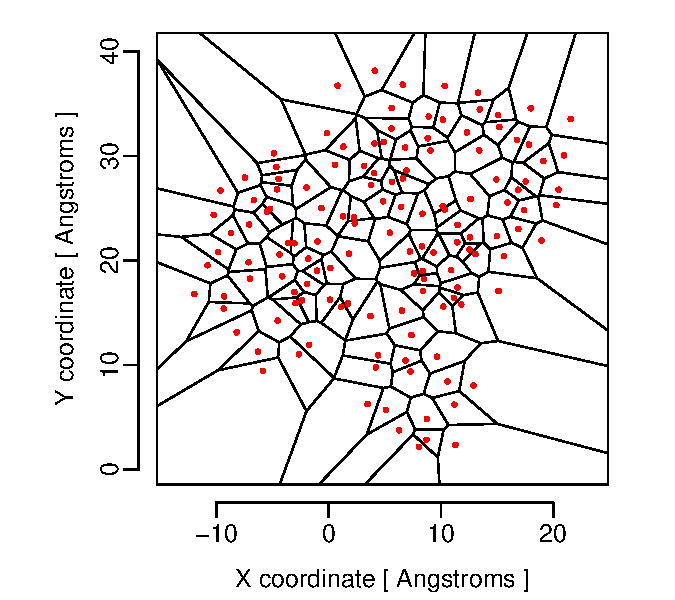
\includegraphics[width=6.9in]{voronoi_diagram.pdf}
        \end{center}
        \caption{Example 2-dimensional Voronoi diagram for bacteriophage T7 lysozyme (Protein Data Bank ID `1LBA'). The red dots represent the backbone $C_\alpha$ atoms projected on the X--Y plane, used as cell seeds in Voronoi tesellation.}
        \label{fig:voronoi}
    \end{figure}


    \begin{figure}[tbh]
        \begin{center}
        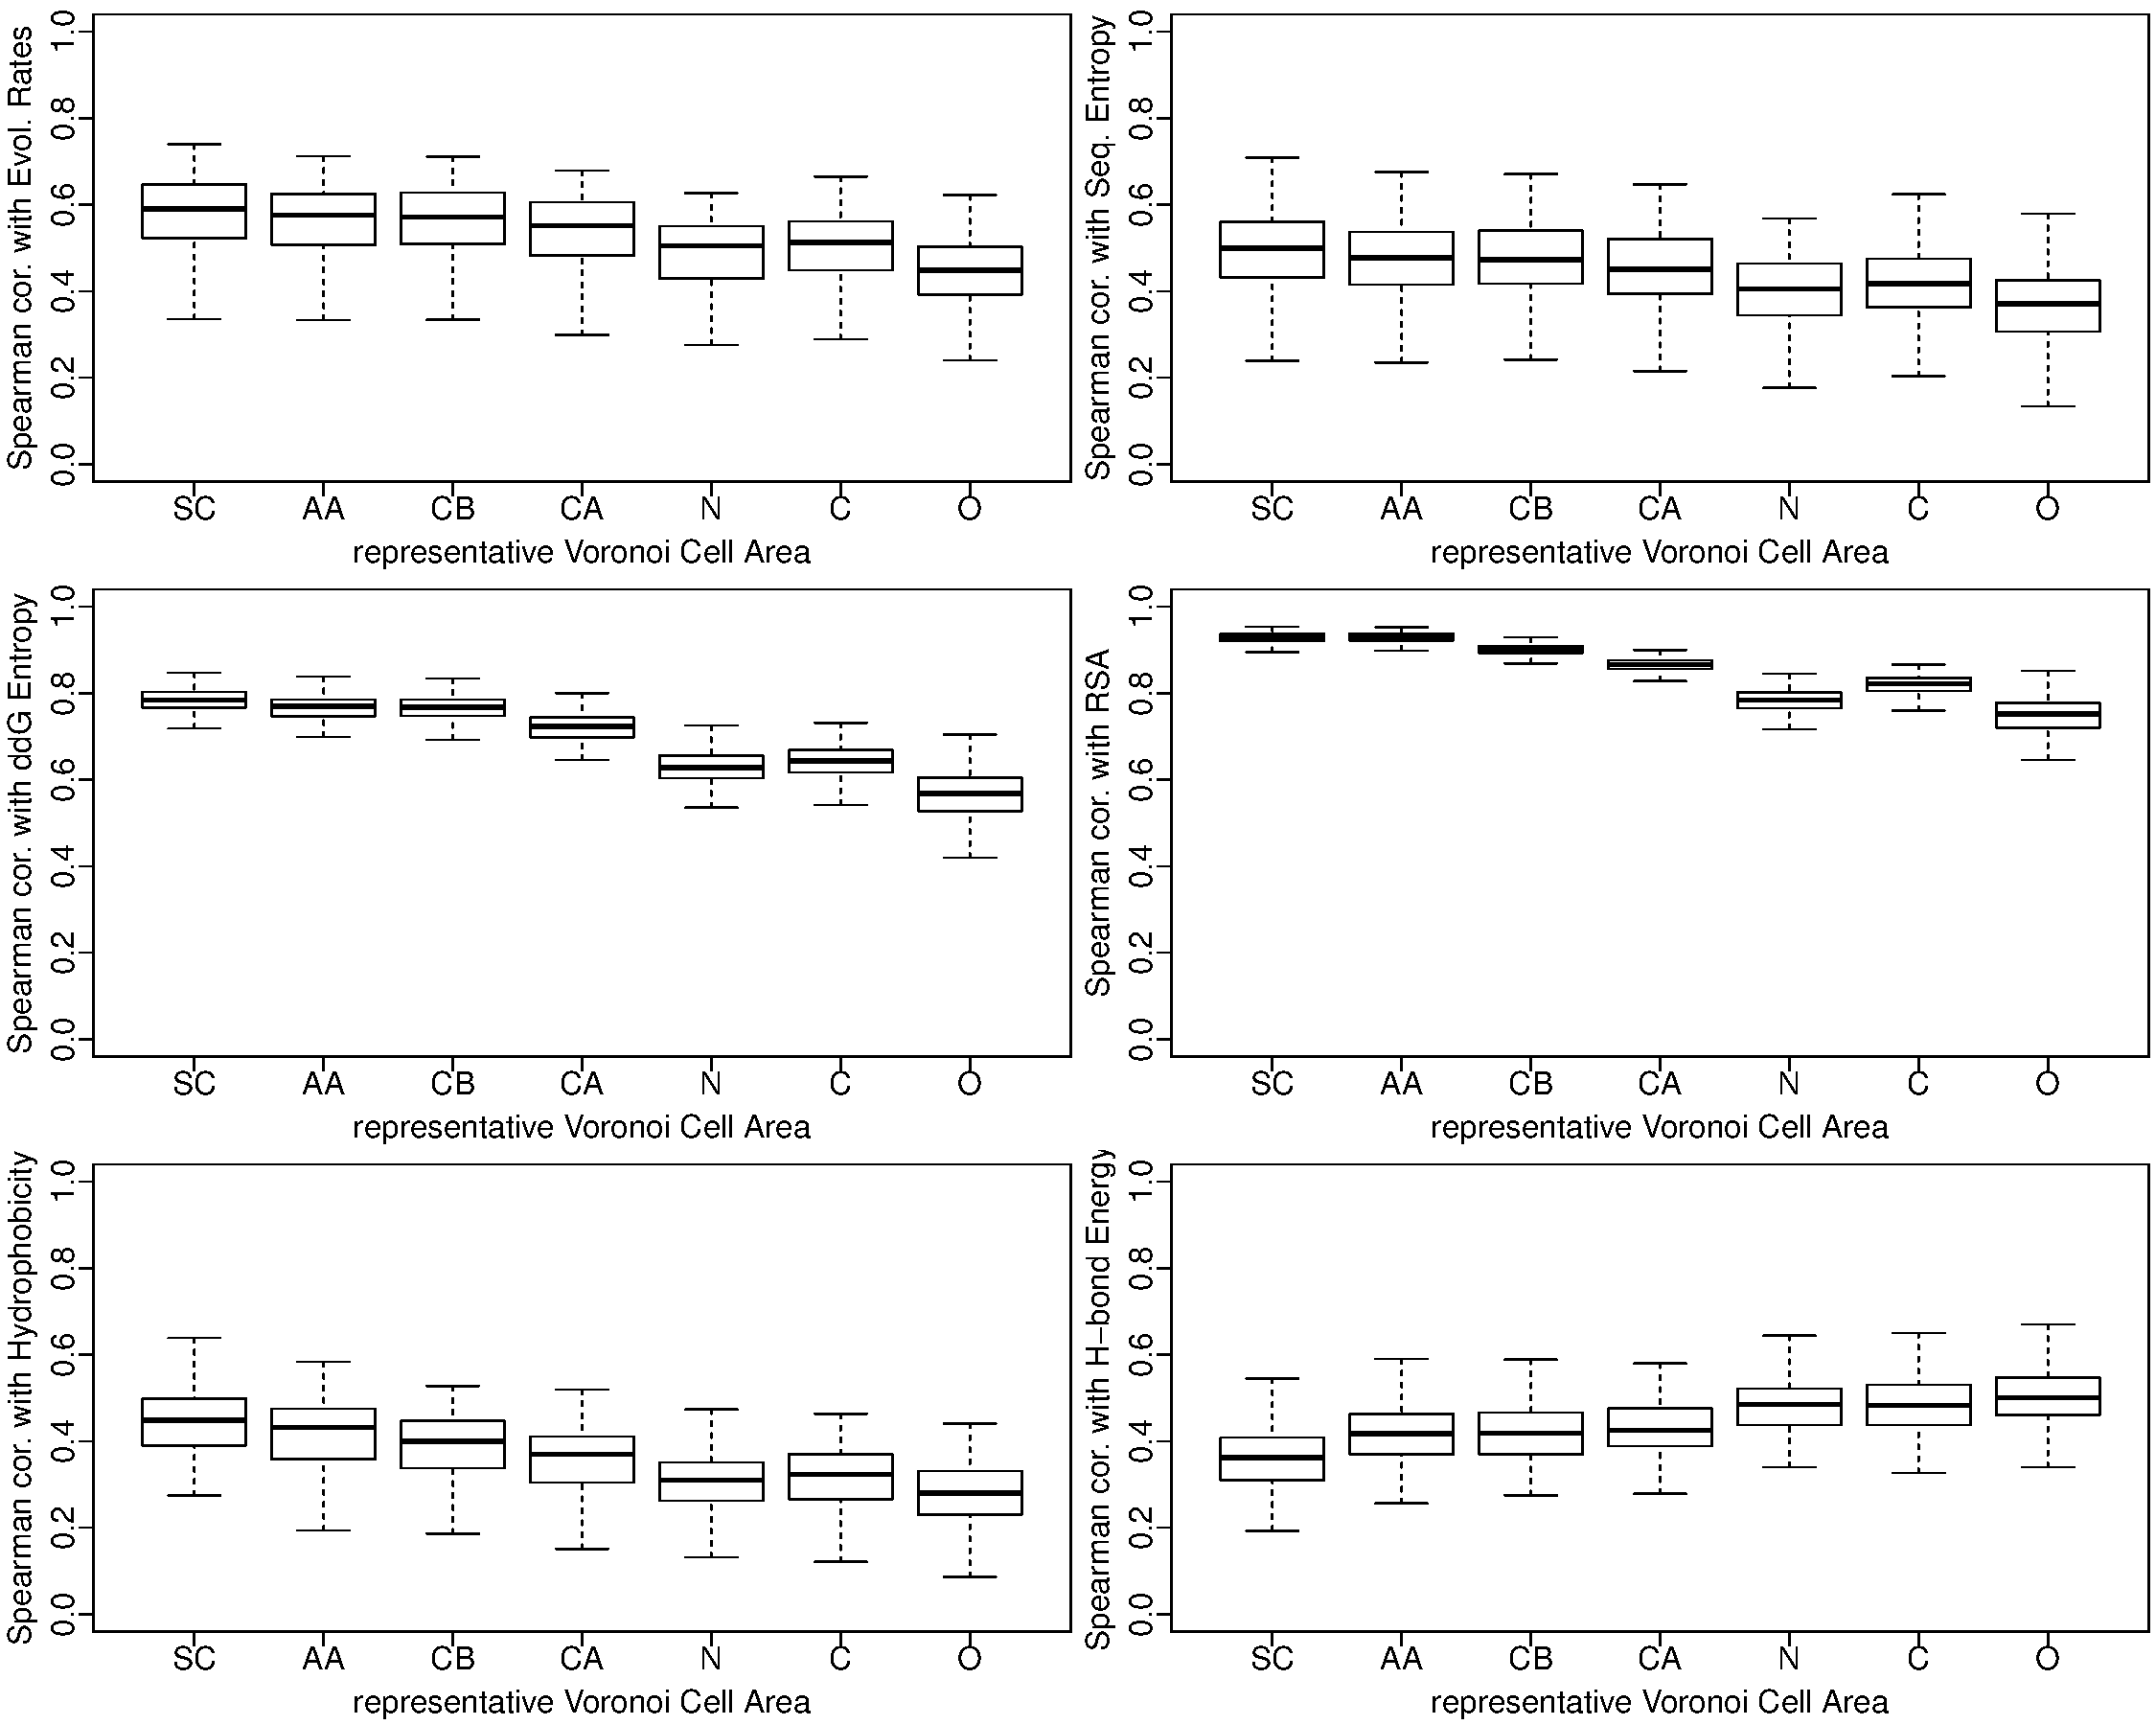
\includegraphics[width=6.9in]{best_varea/select_variables/boxplot_varea_all_in_one.pdf}
        \end{center}
        \caption{A comparison of the correlation strength of 6 different measures of Voronoi cell areas with 6 coordinate-independent structural or sequence properties for 209 proteins in dataset.  The Voronoi cells are generated using 6 sets of atomic coordinates: {\it SC, AA, CB, CA, N, C, O}, used as different representations of individual sites in proteins. The two labels {\it SC} \& {\it AA} stand respectively for the geometric average coordinates of the Side Chain (SC) atoms and the entire Amino Acid (AA) atoms, excluding hydrogens.}
        %about different structure or sequence properties for 209 proteins in dataset. In each plot, the Spearman correlation strengths of a given structure/sequence property on the vertical axis with different measures of cell areas with different atomic Voronoi seeds on the horizontal axis are compared against each other. The capital letters on the horizontal axis denote the set of atomic coordinates used in Voronoi tessellation of protein structures. }
        \label{fig:best_voronoi}
    \end{figure}


    \begin{figure}[tbh]
        \begin{center}
        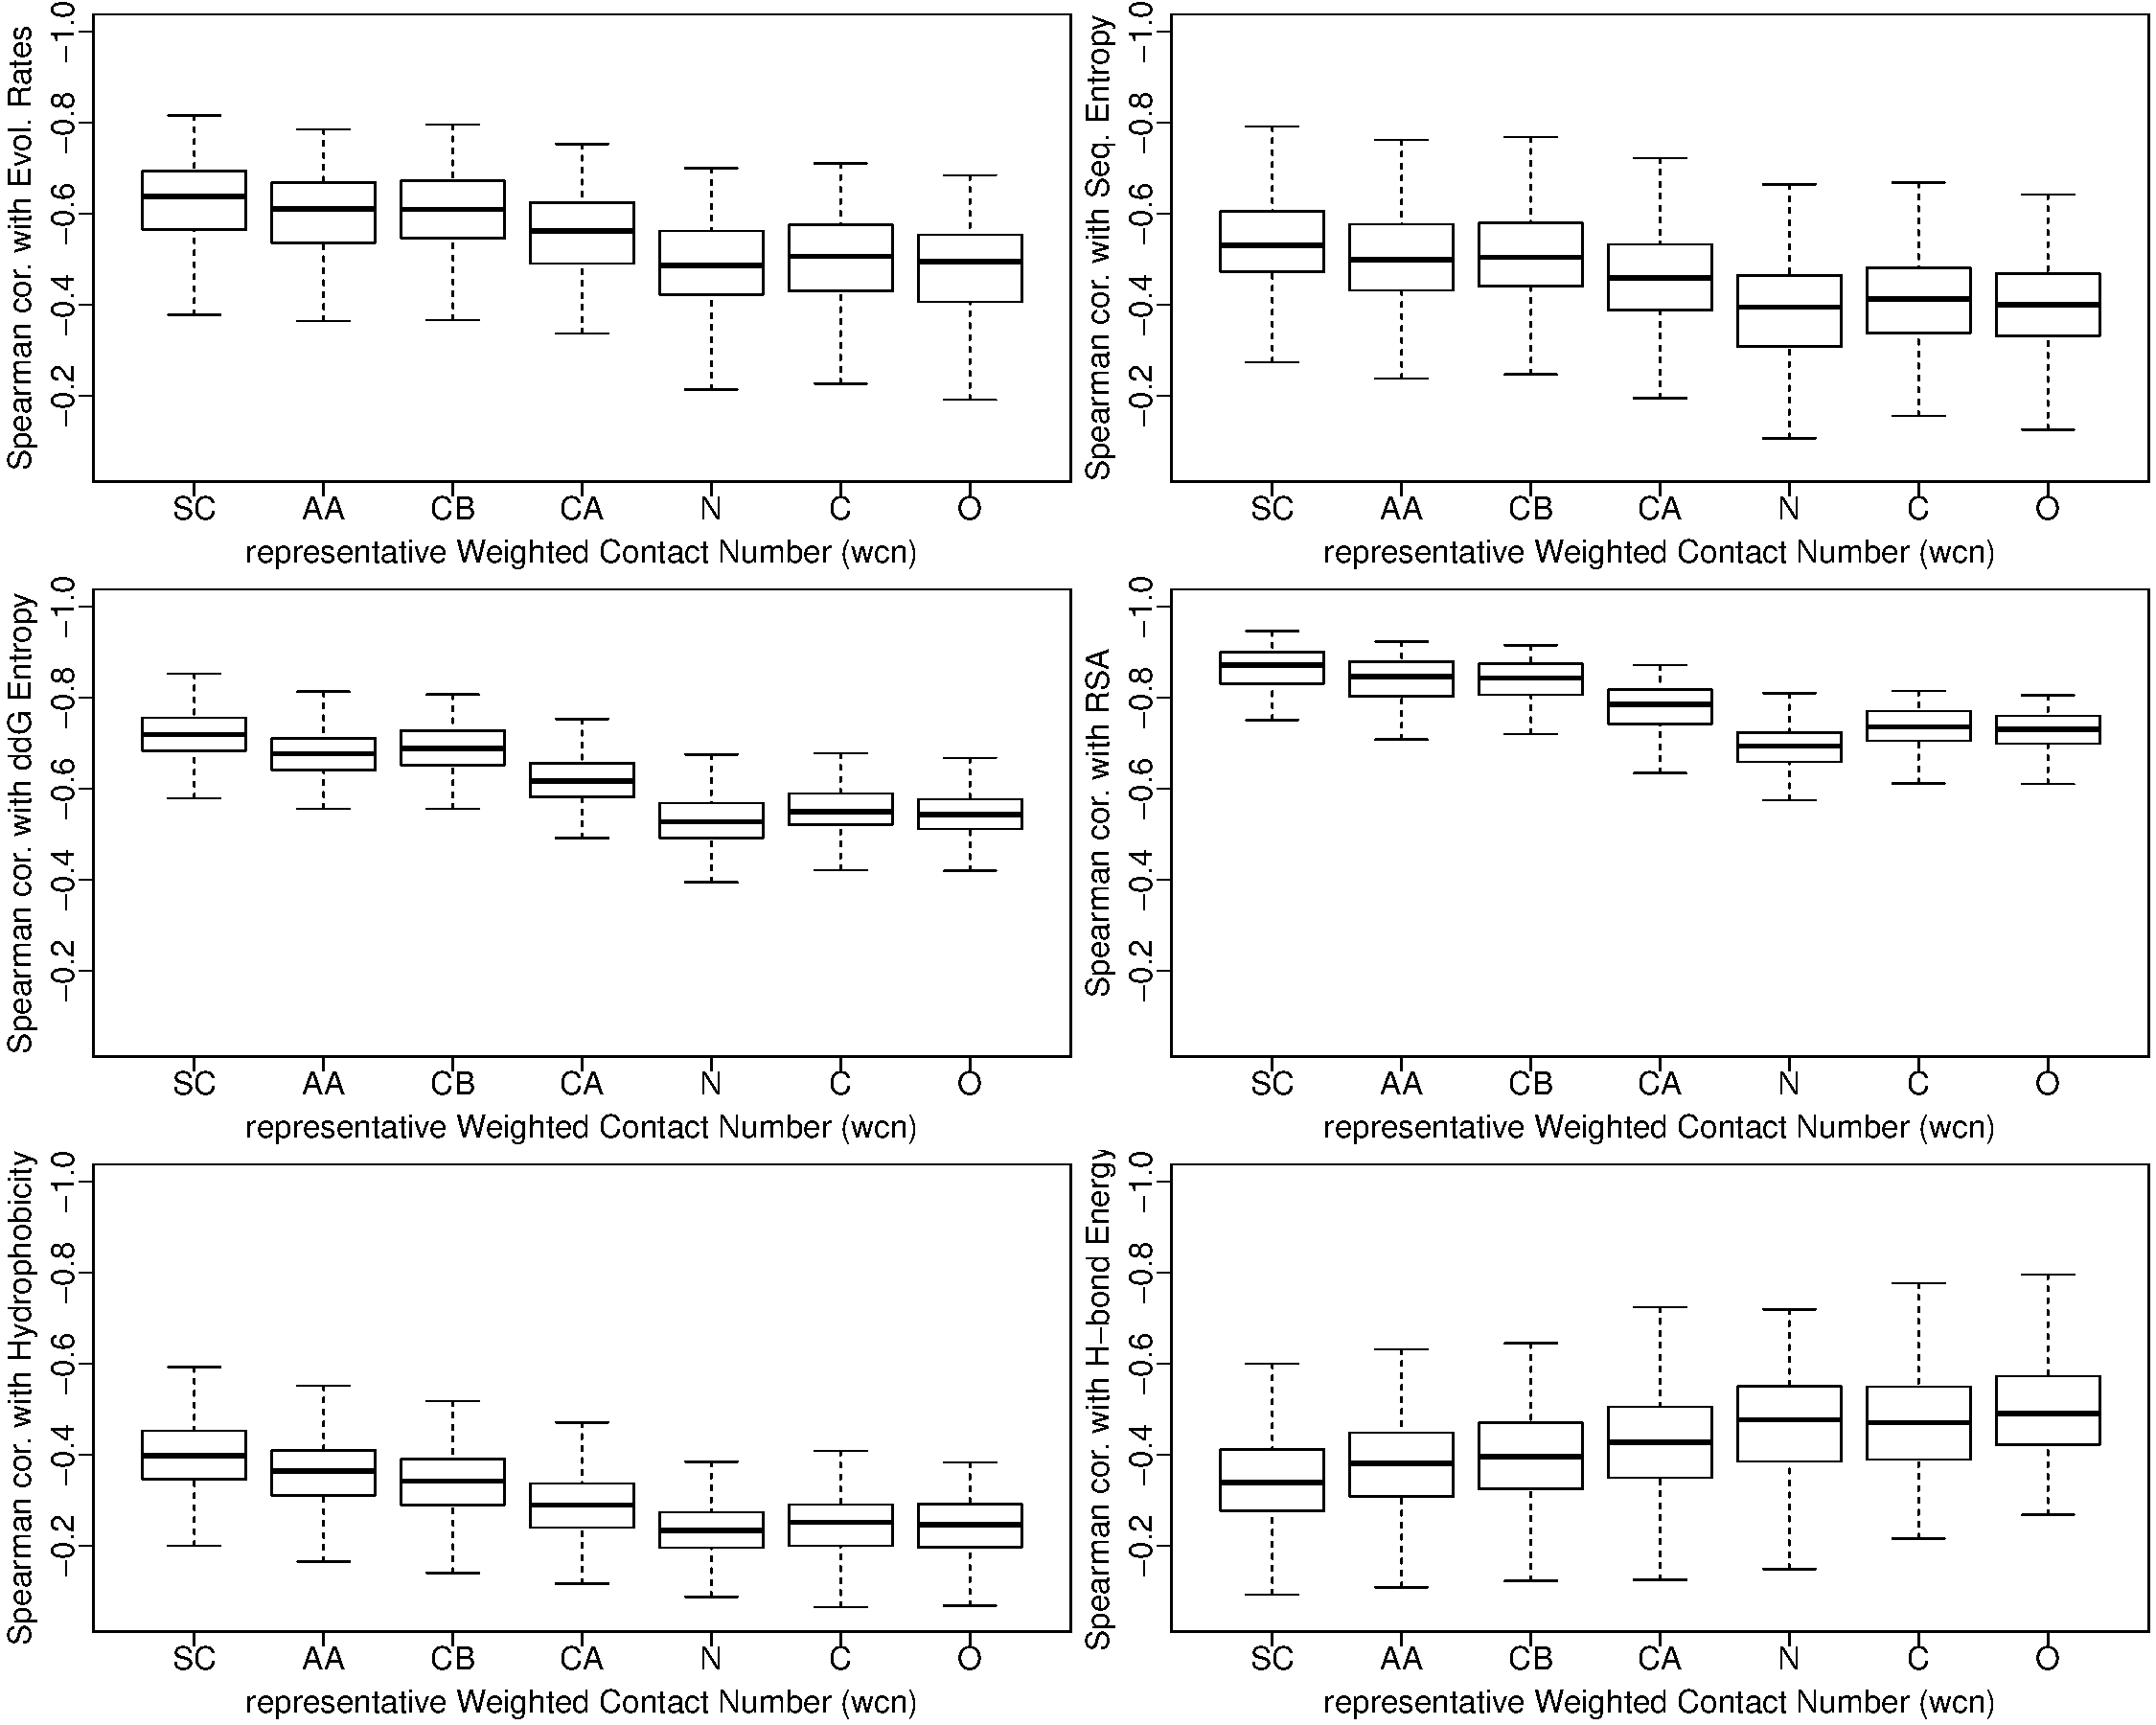
\includegraphics[width=6.9in]{best_wcn/select_variables/boxplot_wcn_all_in_one.pdf}
        \end{center}
        \caption{A comparison of the correlation strength of 6 different measures of Weighted Contact Number (WCN) with 6 coordinate-independent structural or sequence properties for 209 proteins in dataset. The contact numbers, WCN, are calculated using 6 sets of atomic coordinates: {\it SC, AA, CB, CA, N, C, O}, used as different representations of individual sites in proteins. The two labels {\it SC} \& {\it AA} stand respectively for the geometric average coordinates of the Side Chain (SC) atoms and the entire Amino Acid (AA) atoms, excluding hydrogens.}
        \label{fig:best_wcn}
    \end{figure}

    \begin{figure}[tbh]
        \begin{center}
        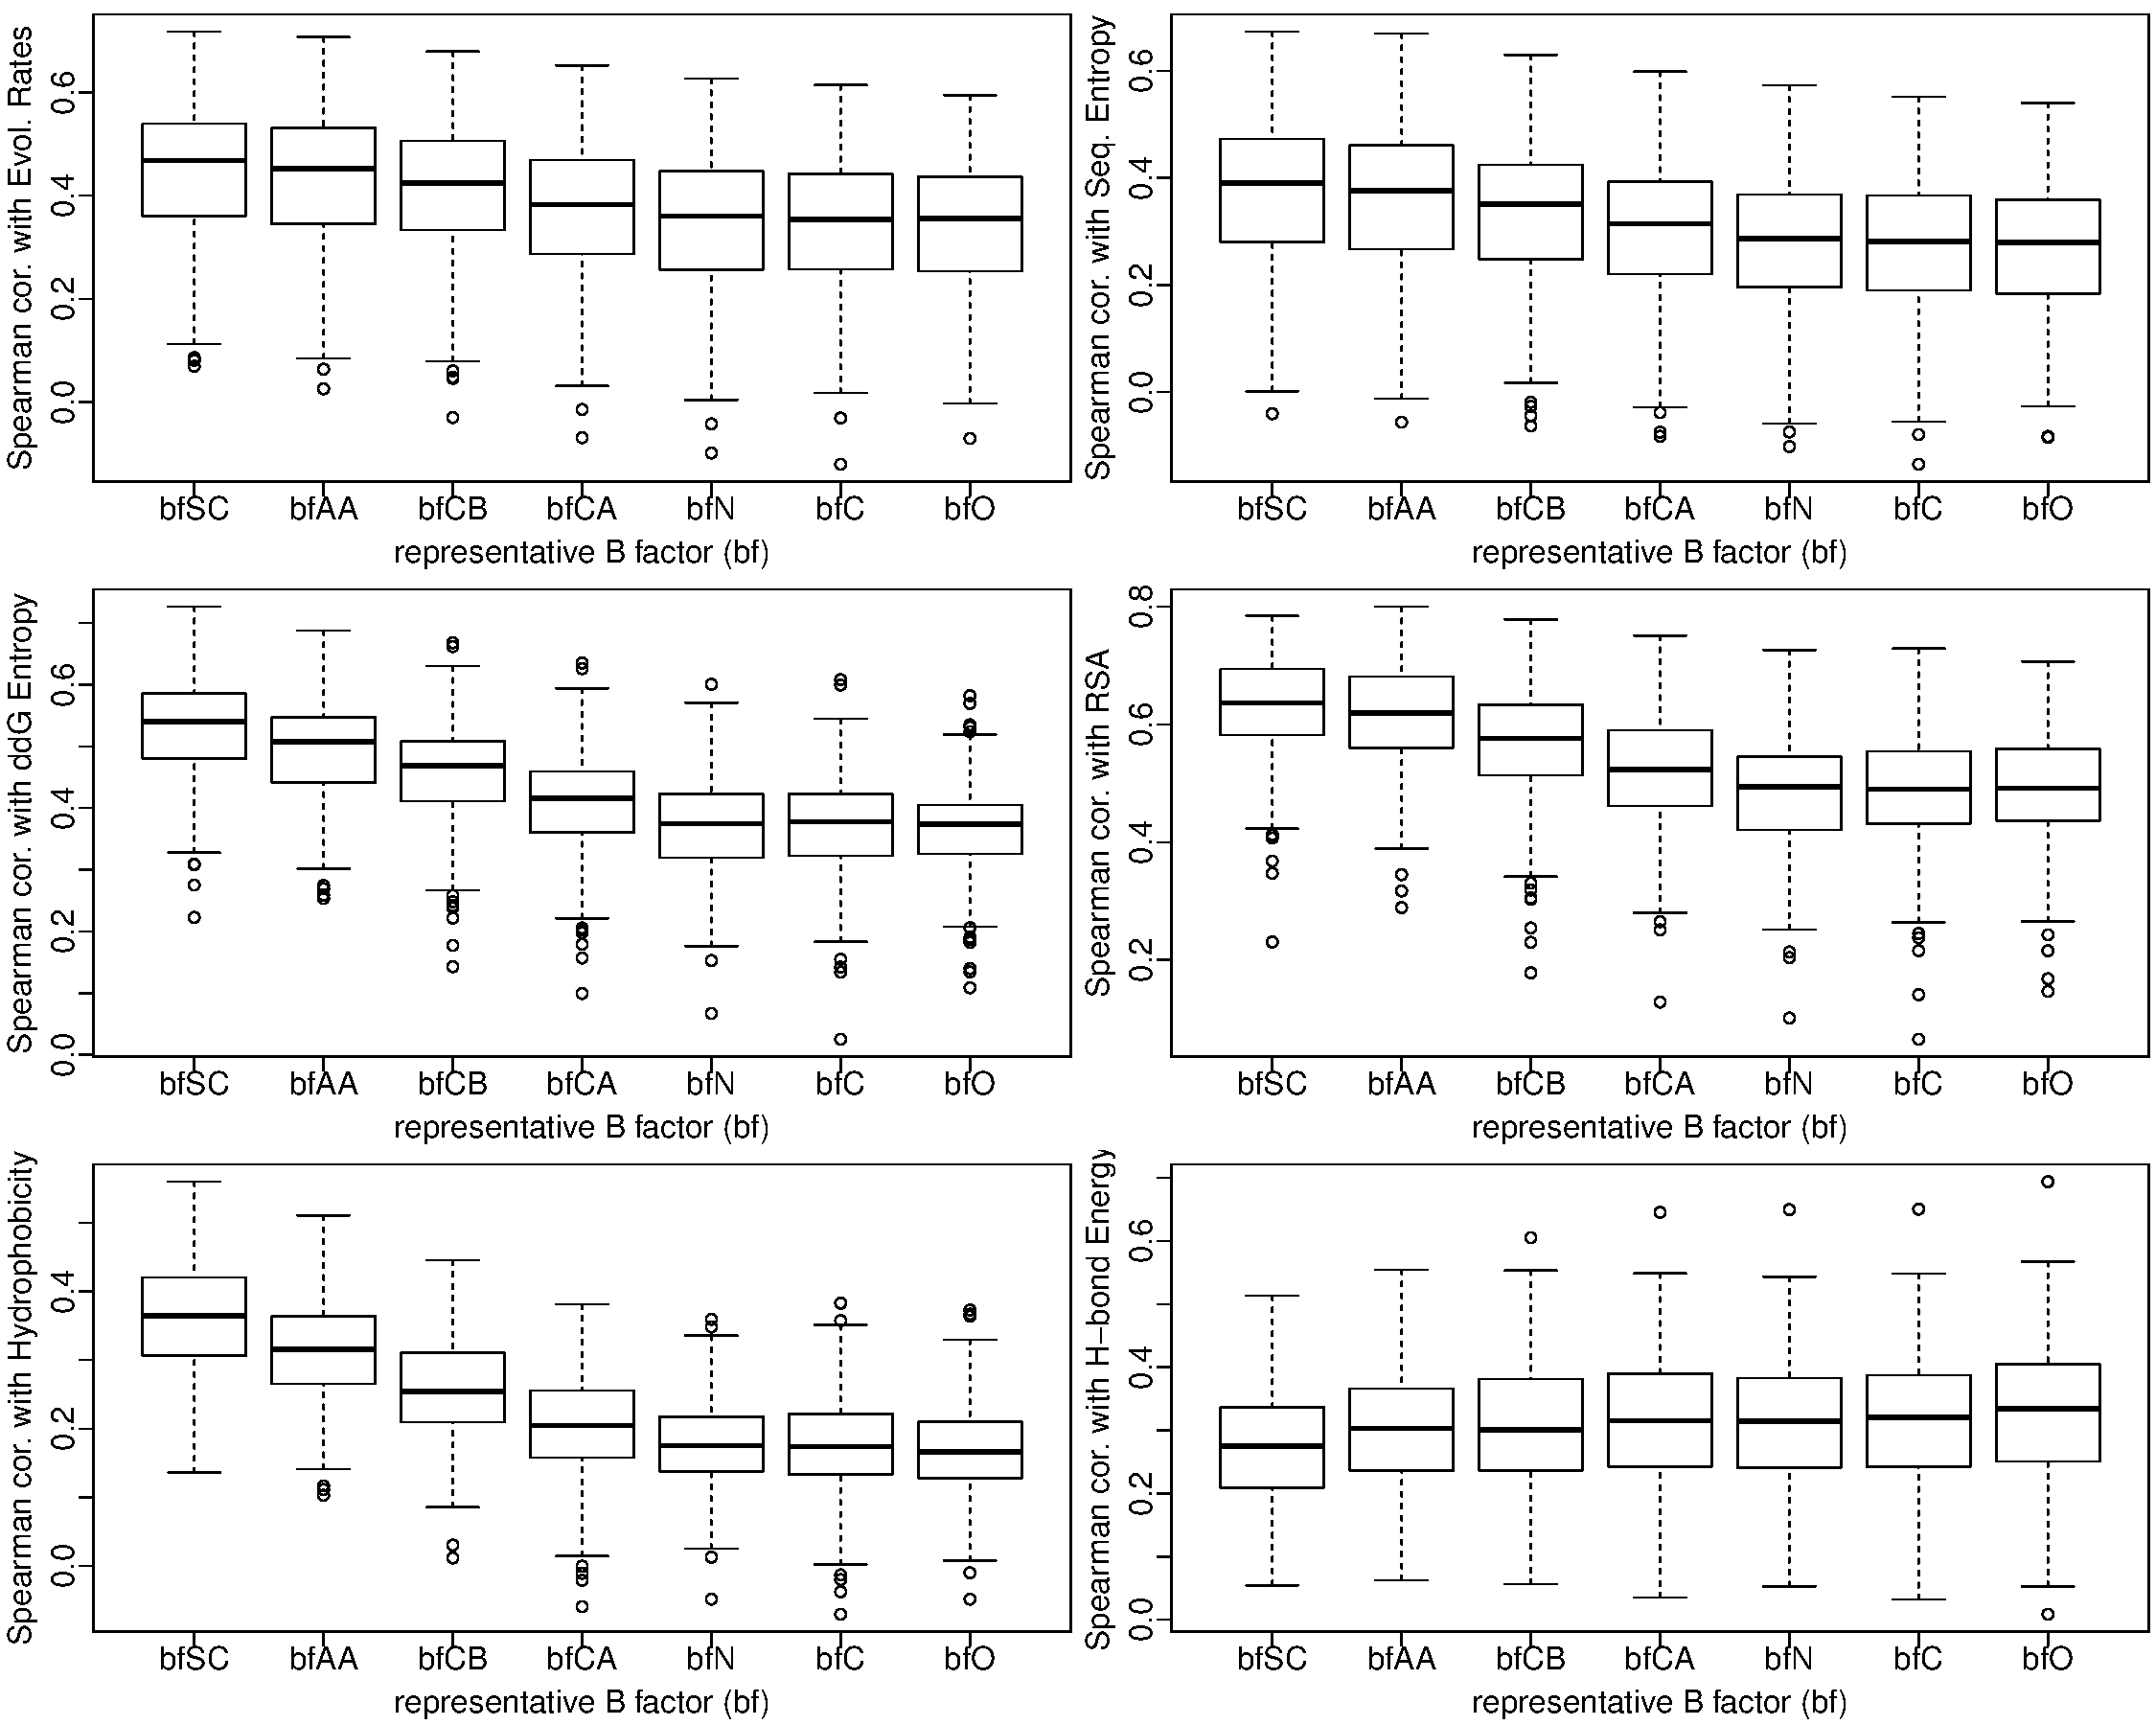
\includegraphics[width=6.9in]{best_bf/select_variables/boxplot_bf_all_in_one.pdf}
        \end{center}
        \caption{A comparison of the correlation strength of 6 different measures of B factor with 6 coordinate-independent structural or sequence properties for 209 proteins in dataset. Shown on the horizontal axes, are the 6 representative atomic B factors: {\it SC, AA, CB, CA, N, C, O} used as flexibility measures of individual sites in proteins. The two variables {\it SC} \& {\it AA} stand respectively for the average B factor of all Side Chain (SC) atoms and the entire Amino Acid (AA) atoms, excluding hydrogens.}
        \label{fig:best_bf}
    \end{figure}

    \begin{figure}[tbh]
        \begin{center}
        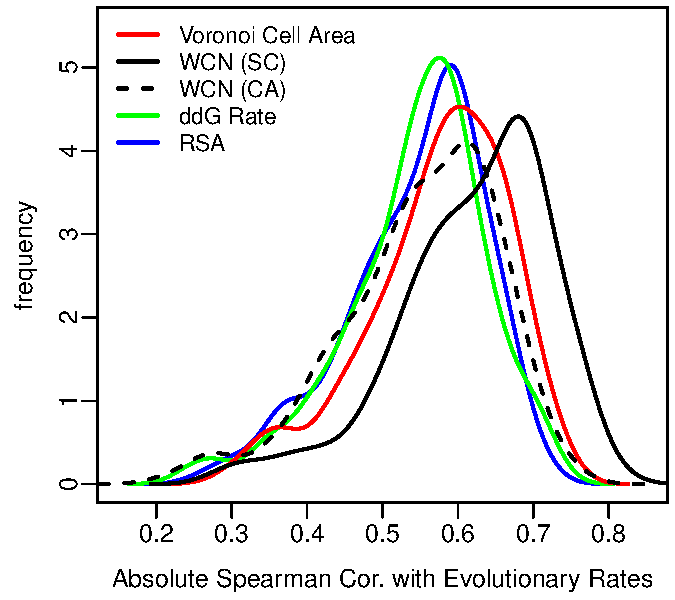
\includegraphics[width=6.9in]{best_structural_predictors_of_ER.pdf}
        \end{center}
        \caption{A comparison of the prediction power of four structural variables about site-specific evolutionary rates. Example 2-dimensional Voronoi diagram for bacteriophage T7 lysozyme (Protein Data Bank ID `1LBA'). The red dots represent the backbone $C_\alpha$ atoms projected on the X--Y plane, used as cell seeds in Voronoi tesellation.}
        \label{fig:best_predictor}
    \end{figure}

%    \begin{figure}[tbh]
%        \begin{center}
%        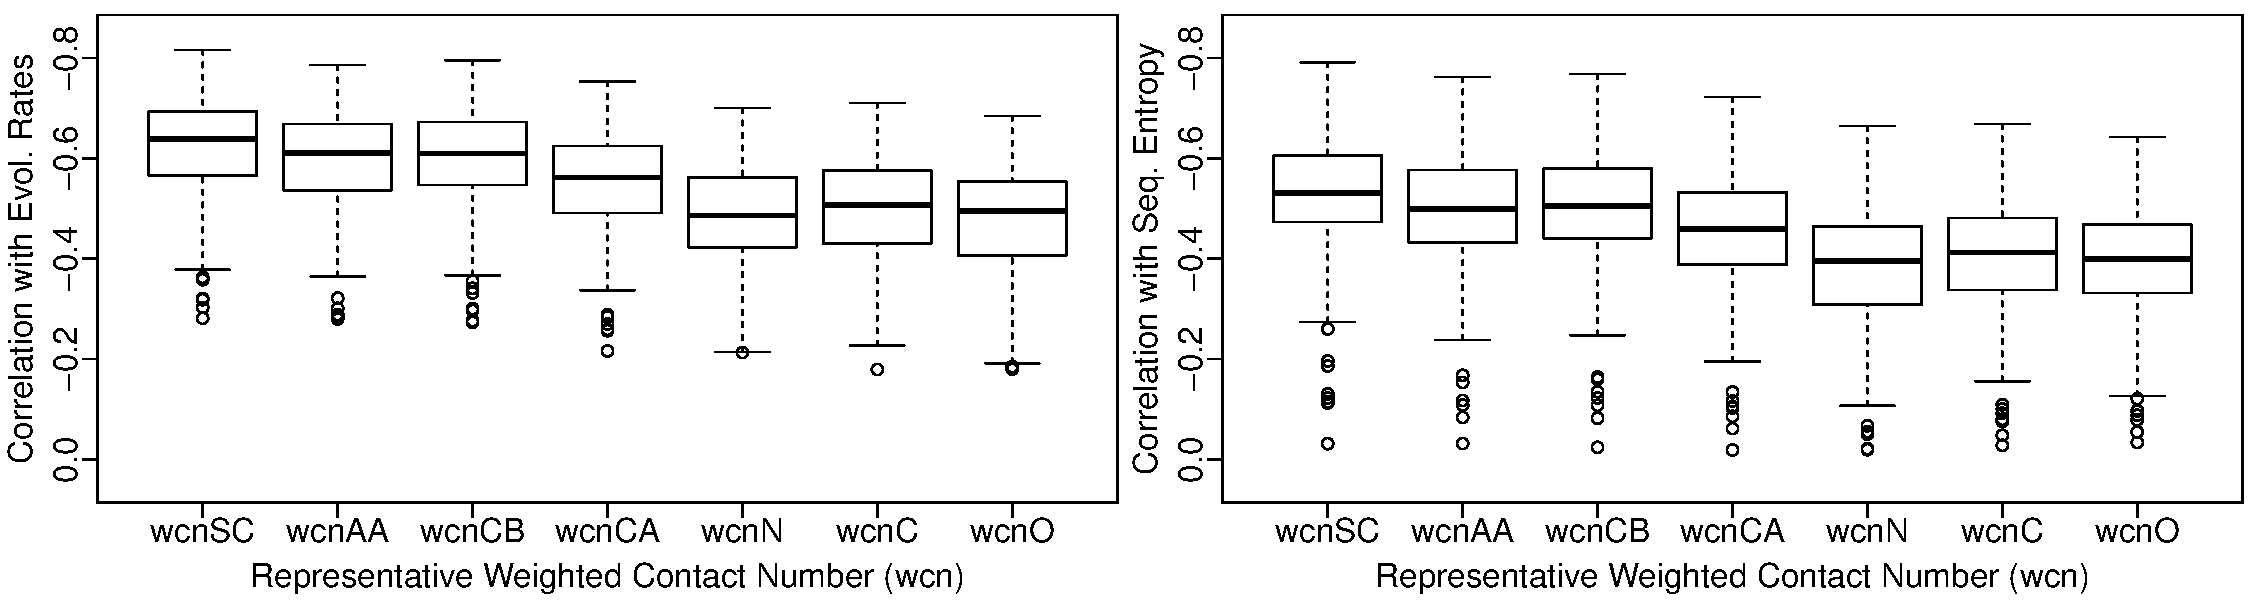
\includegraphics[width=6.9in]{best_wcn/select_variables/boxplot_wcn_two_in_one.pdf}
%        \end{center}
%        \caption{A comparison of the predictive power of different measures of Weighted Contact Number (WCN) about different structure or sequence properties for 209 proteins in dataset. In each plot, the Spearman correlation strengths of a given structure or sequence property on the vertical axis with different measures of WCN on the horizontal axis are compared against each other. The capital letters in the variable names on the horizontal axis denote the set of atomic coordinates used to calculate WCN. The variable $wcnSC$ denotes WCN measure based on the average coordinates over all heavy atoms in the side chain and the variable $wcnAA$ denotes WCN measure based on the average coordinate over all heavy atoms in the side chain and backbone of the amino acid.}
%        \label{fig:best_wcn}
%    \end{figure}

\bibliographystyle{apj}
\bibliography{proc}

\end{document}

